\documentclass[ignorenonframetext]{beamer}
\usetheme{sts}
\usepackage{graphicx}
\usepackage{tikz}
\usetikzlibrary{arrows.meta, positioning}
\usepackage[linesnumbered,ruled,vlined]{algorithm2e}
\title[Data Race Detection]{Static Detection of Data Races in Interrupt-Driven Software Using Reduced Inter-Procedural Control Flow Graphs}

\author{Robin Willenbrock}
\institute{Institute for Software Systems}
\date{\today}

\begin{document}

\begin{document}
\newcommand{\slide1}{%
\begin{frame}<presentation>[plain]
\titlepage{}
\end{frame}
}
\begin{frame}[t]
	\frametitle{Problem of Data Races}
	
	\begin{itemize}
		\item Consequences: Data corruption, security vulnerabilities, system crashes
		\item Not reconstructable or predictable
		\item Real examples of data races:
	\end{itemize}
	
	\vspace{0.5cm} % Adjust the vertical space as needed
	
	\begin{tabular}{p{0.48\textwidth} p{0.48\textwidth}}
		\begin{flushleft}
			% Content for the left side
			\centering \textbf{Therac-25 Incident} \\[0.2cm]
			\raggedright % Make the following text left-aligned
				\begin{figure}
					\centering
					
\includegraphics[width=3\linewidth]{Files/DataCorruption}
					\caption{}
					\label{fig:datacorruption}
				\end{figure}
		\end{flushleft} &
		\begin{flushleft}
			% Content for the right side
			\centering \textbf{Kubernetes Server Vulnerability} \\[0.2cm]
			\raggedright % Make the following text left-aligned
				\begin{figure}
					\centering
					
\includegraphics[width=3.1\linewidth]{Files/Securitybreach}
					\caption{}
					\label{fig:securitybreach}
				\end{figure}
		\end{flushleft}
	\end{tabular}
\end{frame}


\begin{frame}<presentation>
\frametitle{Contents}
%\tableofcontents[hideallsubsections]{}
\tableofcontents[]{}
\end{frame}
}

\section{Data Races}
\begin{frame}[t]
\frametitle{What are Data Races?}
		\begin{tabular}{p{0.48\textwidth} p{0.48\textwidth}}
		\begin{flushleft}
			% Content for the left side
			\centering \textbf{Interrupt Driven Systems} \\[0.2cm]
			\raggedright % Make the following text left-aligned
			\begin{figure}
				\centering
				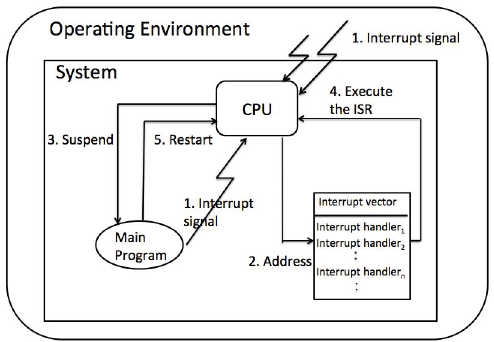
\includegraphics[width=0.5\textwidth]{../../Presentation/beamer/Files/The-Mechanism-of-Interrupt}
				\caption{Interrupt Driven System}
				\label{fig:the-mechanism-of-interrupt}
			\end{figure}
		\end{flushleft} &
	
	\end{tabular}
\end{frame}
\begin{frame}[t]
	\frametitle{What are Data Races?}
	\begin{tabular}{p{0.48\textwidth} p{0.48\textwidth}}
		\begin{flushleft}
			% Content for the left side
			\centering \textbf{Interrupt Driven Systems} \\[0.2cm]
			\raggedright % Make the following text left-aligned
			\begin{figure}
				\centering
				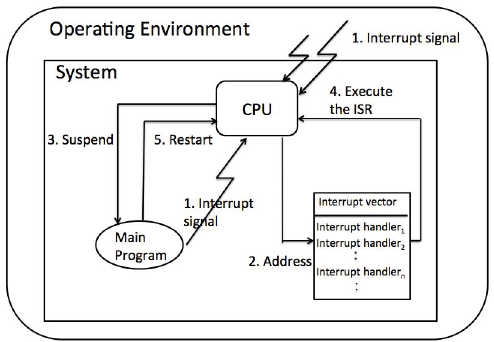
\includegraphics[width=0.5\textwidth]{../../Presentation/beamer/Files/The-Mechanism-of-Interrupt}
				\caption{Interrupt Driven System}
				\label{fig:the-mechanism-of-interrupt}
			\end{figure}
		\end{flushleft} &
		\begin{flushleft}
			% Content for the right side
			\centering \textbf{Shared Resources} \\[0.2cm]
			\raggedright % Make the following text left-aligned
			\vspace{0.8cm}
			\begin{figure}
			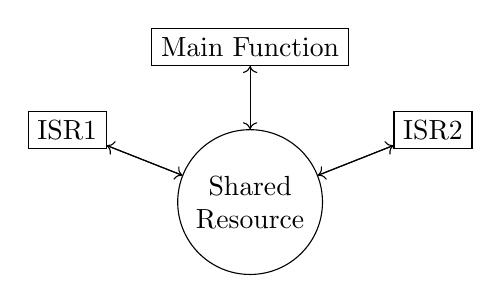
\begin{tikzpicture}[node distance=0.8cm, every node/.style={align=center}]
				% Nodes
				\node (main) [rectangle, draw] {Main Function};
				\node (isr1) [rectangle, draw, below left=of main] {ISR1};
				\node (isr2) [rectangle, draw, below right=of main] {ISR2};
				\node (shared) [circle, draw, below=of main] {Shared\\Resource};
				
				% Arrows
				\draw[->] (main) -- (shared);
				\draw[->] (isr1) -- (shared);
				\draw[->] (isr2) -- (shared);
				\draw[->] (shared) -- (main);
				\draw[->] (shared) -- (isr1);
				\draw[->] (shared) -- (isr2);
			\end{tikzpicture}
			\end{figure}
		\end{flushleft}
	\end{tabular}
\end{frame}

\begin{frame}
	\frametitle{What are Data Races?}
\begin{figure}
	\centering
	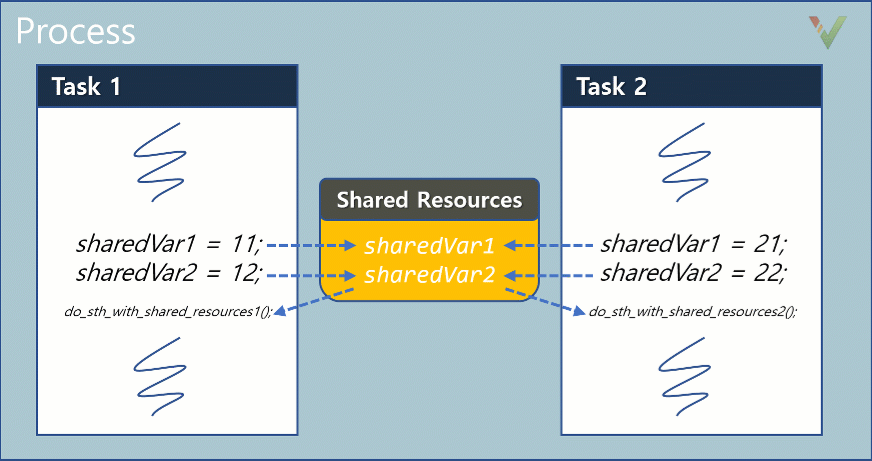
\includegraphics[width=0.8\textwidth]{../../Presentation/beamer/Files/Data Races} % Adjust the width as needed
	\caption{Data Races}
	\label{fig:data-races}
\end{figure}

\end{frame}
\begin{frame}
\frametitle{Example of a Data Race}
\begin{algorithm}[H]
	\caption{Example 1}
	\KwData{long shared1;}
	
	\BlankLine
	\SetKwFunction{FMain}{main}
	\SetKwProg{Fn}{Function}{:}{}
	\Fn{\FMain()}{
		\BlankLine
		\textbf{Variables}:\\
		unsigned char tmp\;
		\BlankLine
		\textbf{Code}:\\
		tmp $\leftarrow$ shared1\;
	}
	
	\BlankLine
	\SetKwFunction{FIsr}{isr1}
	\Fn{\FIsr()}{
		\BlankLine
		\textbf{Code}:\\
		idlerun()\;
		shared1 $\leftarrow$ 1\;
		idlerun()\;
	}
\end{algorithm}
\end{frame}
\begin{frame}[t]
	\frametitle{Static Detection}
	\begin{tabular}{p{0.48\textwidth} p{0.48\textwidth}}
	\begin{flushleft}
		% Content for the left side
		\centering \textbf{Upsides} \\[0.2cm]
		\raggedright % Make the following text left-aligned
		\begin{itemize}
			\item Code-based
			\item Scalability
			\item Detection in development process
		\end{itemize}
	\end{flushleft} &
	\begin{flushleft}
		% Content for the right side
		\centering \textbf{Downsides} \\[0.2cm]
		\raggedright % Make the following text left-aligned
		\begin{itemize}
			\item False positives
			\item Results need to be interpreted
		\end{itemize}
	\end{flushleft}
\end{tabular}
\end{frame}
\begin{frame}
	\frametitle{How to detect Data Races}
	\begin{algorithm}[H]
		\caption{Static Race Detection}
		\KwIn{RICFGs of P}
		\KwOut{potential racing pairs (PR)}
		
		\BlankLine
		\For{each $< G_i ; G_j >$ in RICFGs}{
			\For{each $sv_i \in G_i$}{
				\For{each $sv_j \in G_j$}{
					\If{$sv_i.V == sv_j.V$ and $(sv_i.A == W$ or $sv_j.A == W)$ and $G_i.pri < G_j.pri$ and $INTB.get(svi).contains(Gj)$}{
						$PR = PR \cup \{ <sv_i, sv_j> \}$\;
					}
				}
			}
		}
	\end{algorithm}
\end{frame}
\section{Control Flow Graph}
\begin{frame}[t]
	\frametitle{Why do we need Control Flow Graphs?}
	\scriptsize % Adjust font size to fit content
	\tiny
	\begin{algorithm}[H]
		\caption{Example 2}
		\KwData{long shared1}
		
		\SetKwFunction{FMain}{main}
		\SetKwProg{Fn}{Function}{:}{}
		
		\Fn{\textbf{main()}}{
			\textbf{Variables}:\\
			unsigned char tmp\;
			\BlankLine
			\textbf{Code}:\\
			disable\_isr(1)\;
			\If{shared1 == 0}{
				enable\_isr(1)\;
			}
			\Else{
				int variable2 = 1\;
			}
			tmp $\leftarrow$ shared1\;
			enable\_isr(1)\;
		}
		
		\Fn{\textbf{isr1()}}{
			\textbf{Code}:\\
			idlerun()\;
			shared1 $\leftarrow$ 1\;
			idlerun()\;
		}
		
		\Fn{\textbf{isr2()}}{
			\textbf{Code}:\\
			idlerun()\;
			int variable1 = 1\;
			idlerun()\;
		}
	\end{algorithm}
\end{frame}
\begin{frame}
	\frametitle{What are Inter-Procedural CFG's?}
	\begin{tabular}{p{0.48\textwidth} p{0.48\textwidth}}
	\begin{flushleft}
		\raggedright % Make the following text left-aligned
		\begin{itemize}
			\item Using information of all functions
			\item Potential interrupts at any points need to be considered
			\item Analysing each CFG alone would not show all potential races
			\item Example: Potential interrupts from isr1 here must be considered at any given time
		\end{itemize}
	\end{flushleft} &
	\begin{flushleft}
		\raggedright % Make the following text left-aligned
		\begin{figure}
			\centering
			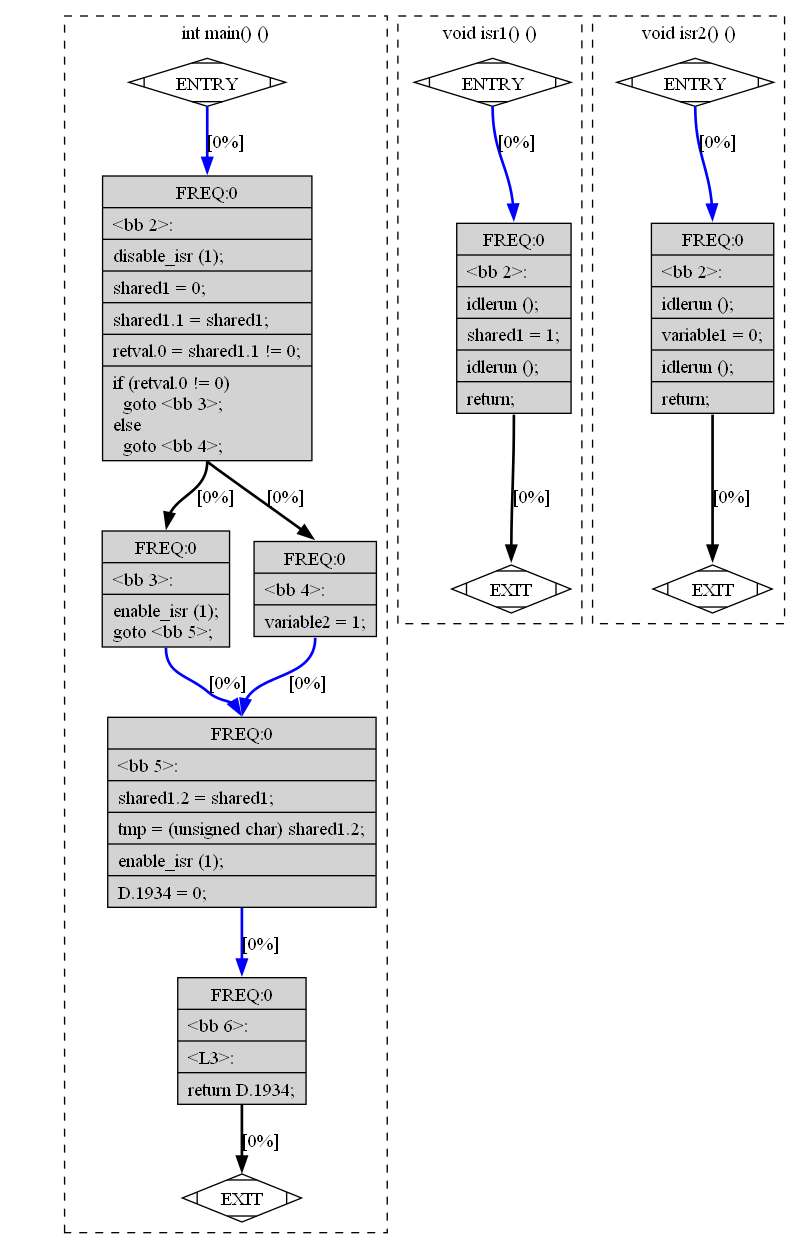
\includegraphics[height=0.8\textheight]{../../Presentation/beamer/Files/VortragCFG}
			\caption{Full CFG}
			\label{fig:vortragcfg}
		\end{figure}
	\end{flushleft}
	\end{tabular}
	\end{frame}
\begin{frame}
	\frametitle{Reducing the CFG}
	\begin{tabular}{p{0.48\textwidth} p{0.48\textwidth}}
		\begin{flushleft}
			\raggedright % Make the following text left-aligned
			\begin{figure}
				\centering
				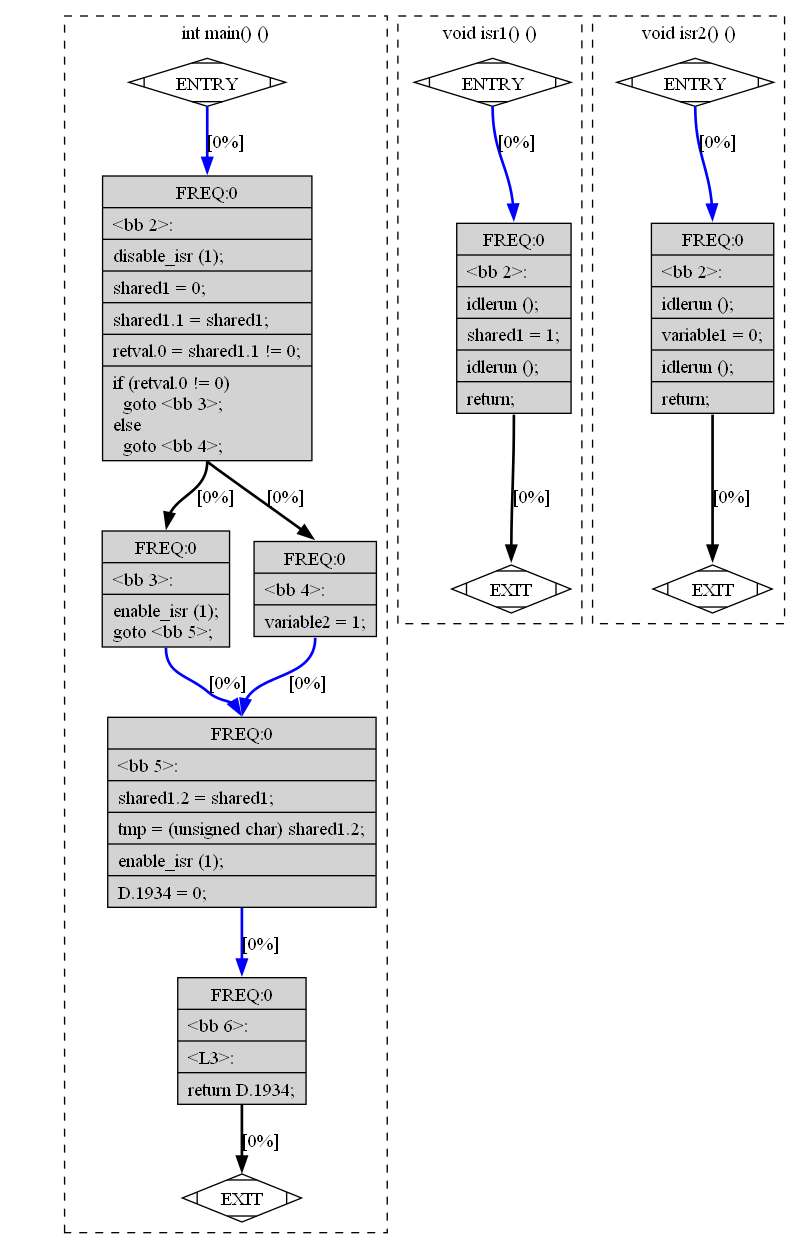
\includegraphics[height=0.6\textheight]{../../Presentation/beamer/Files/VortragCFG}
				\caption{Full CFG}
				\label{fig:vortragcfg}
			\end{figure}
		\end{flushleft} &
		\begin{flushleft}
			\raggedright % Make the following text left-aligned
			\begin{figure}
				\centering
				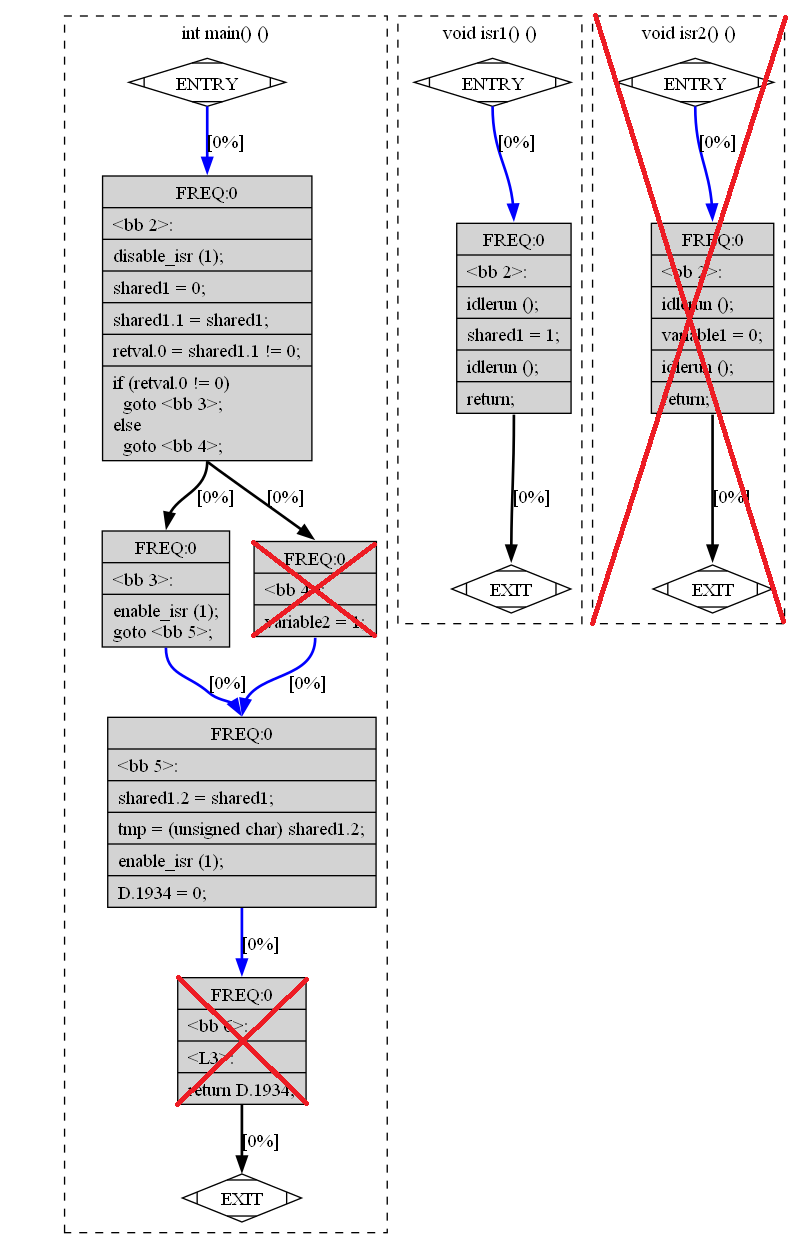
\includegraphics[height=0.6\textheight]{../../Presentation/beamer/Files/VortragReducedCFG}
				\caption{Reduced CFG}
				\label{fig:vortragreducedcfg}
			\end{figure}
		\end{flushleft}
	\end{tabular}
\end{frame}
\section{Interrupt Handling}
\begin{frame}
	\frametitle{Interrupt Status}
	\begin{tabular}{p{0.48\textwidth} p{0.48\textwidth}}
		\begin{flushleft}
			\raggedright % Make the following text left-aligned
			\begin{itemize}
				\item Need an Array to keep track of the enabled/disabled ISR's
				\item Updated after every Basic Block
				\item Special Case: \\
				ISR enabled/disabled by another ISR
			\end{itemize}
		\end{flushleft} &
		\begin{flushleft}
			\raggedright % Make the following text left-aligned
			\begin{figure}
				\centering
				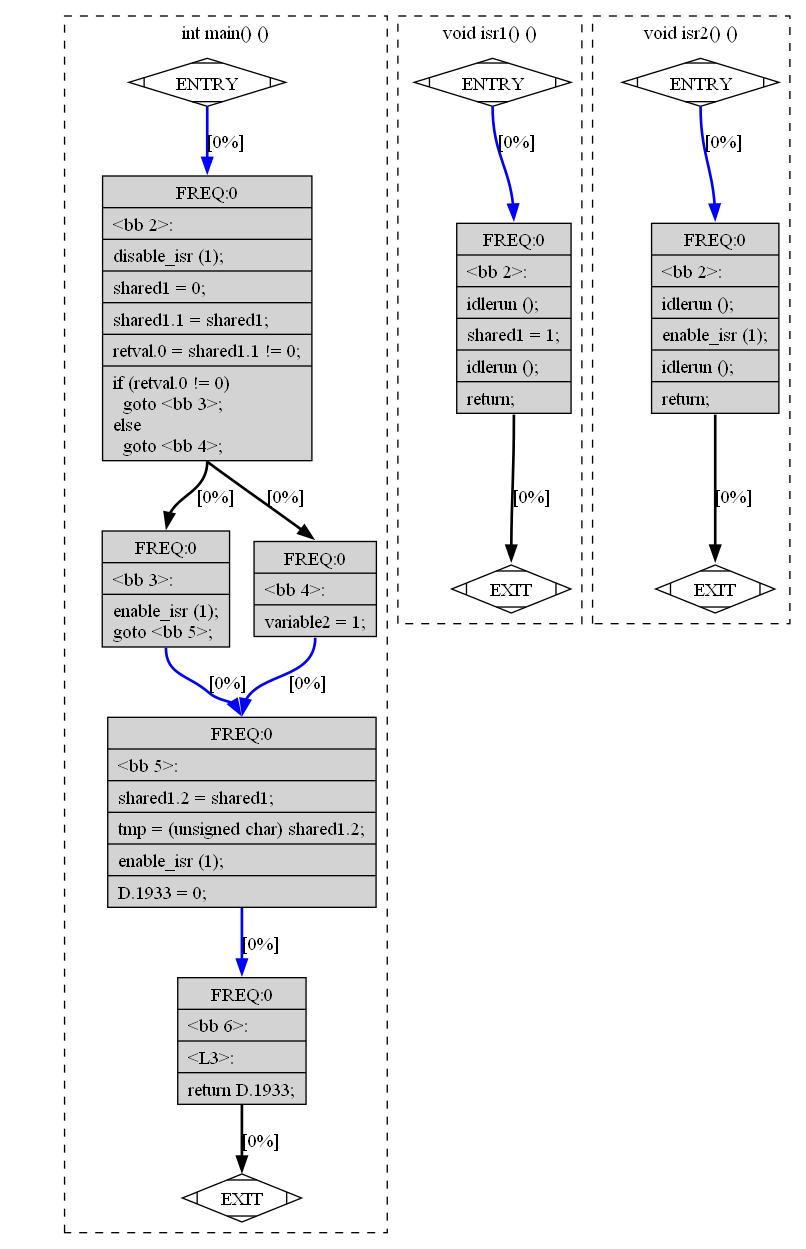
\includegraphics[height=0.8\textheight]{../../Presentation/beamer/Files/VortragCFG2}
				\caption{Full CFG}
				\label{fig:vortragcfg}
			\end{figure}
		\end{flushleft}
	\end{tabular}
	\section{Summary}
\end{frame}
\begin{frame}[fragile]
	\frametitle{Interrupt Enabling/Disabling ISR}
	\scriptsize % Adjust font size to fit content
	\tiny
	\begin{algorithm}[H]
		\caption{Example 3}
		\KwData{long shared1}
		
		\SetKwProg{Fn}{Function}{:}{}
		
		\Fn{\textbf{main()}}{
			\textbf{Variables}:\\
			unsigned char tmp\;
			\BlankLine
			\textbf{Code}:\\
			disable\_isr(1)\;
			\If{shared1 == 0}{
				enable\_isr(1)\;
			}
			\Else{
				int variable2 = 1\;
			}
			tmp $\leftarrow$ shared1\;
			enable\_isr(1)\;
		}
		
		\Fn{\textbf{isr1()}}{
			\textbf{Code}:\\
			idlerun()\;
			shared1 $\leftarrow$ 1\;
			idlerun()\;
		}
		
		\Fn{\textbf{isr2()}}{
			\textbf{Code}:\\
			idlerun()\;
			enable\_isr(1)\;
			idlerun()\;
		}
	\end{algorithm}
\end{frame}
\begin{frame}
\frametitle{Summary}
	\begin{tabular}{p{0.48\textwidth} p{0.48\textwidth}}
		\begin{flushleft}
			% Content for the left side
			\centering \textbf{Solved Problems} \\[0.2cm]
			\raggedright % Make the following text left-aligned
			\begin{itemize}
				\item Detecting data races reliably 
				\item Tracking interrupt status in all states of the programm
				\item Generating a reduced control flow graph and analysing it inter-proceduraly
			\end{itemize}
		\end{flushleft} &
		\begin{flushleft}
			% Content for the right side
			\centering \textbf{Future Work} \\[0.2cm]
			\raggedright % Make the following text left-aligned
			\begin{itemize}
				\item Minimizing the amount of false positives
				\item Automatic detection of shared resources
				\item Further analysis of interrupt enable status
			\end{itemize}
		\end{flushleft}
	\end{tabular}

\end{frame}
\begin{frame}
	\frametitle{Quellen}
	\tiny
	\begin{itemize}
		\item URL: https://nvd.nist.gov/vuln/detail/cve-2018-1002105 Last Updated:29.05.2024 Accessed:06.06.2024
		\item Article: Berühmt berüchtigter Softwarefehler Therac-25 Author: Martin Pfeifer URL: https://formal.kastel.kit.edu/~beckert/teaching/Seminar-Softwarefehler-SS03/Ausarbeitungen/pfeifer.pdf Accessed:06.06.2024
		\item URL: https://github.com/chenruibuaa/racebench Accessed:07.06.2024
		\item Title: Automatic Detection, Validation, and Repair of Race Conditions in Interrupt-Driven Embedded Software Author: Yu Wang et al.
		\item URL: https://www.researchgate.net/figure/The-Mechanism-of-Interrupt Publisher: Huibiao Zhu Accessed: 03.06.2024
		\item URL: https://de.mathworks.com/products/polyspace/static-analysis-notes/what-data-races-how-avoid-during-software-development.html Author: Yoo Yong-chul Publisher: MathWorks Korea Published:17.04.2021 Accessed: 03.06.2024
	\end{itemize}
\end{frame}
\end{document}
